\subsection{Early days of the Internet and its remaining flaws}

The need to build a global communications network in an age when almost nobody had access to technology and the number of future users was unpredictable, caused that some protocols weren't suitable for a huge increase on the amount of publicly known users. \ac{IPv4} limits the number of public addresses in such a way that today is scarce \cite{ipv4}. One way to overcome this problem was the development of a mechanism that groups multiple address into a single one, the machine that is assigned that address is then responsible to redirect messages to members of its group through their private addresses, each member of the private network is identified publicly by the same \ac{IP} address with a different port, this technique is also known as \ac{NAT}.

\begin{figure}[H]
	\centering
	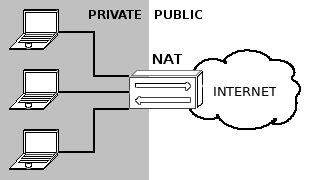
\includegraphics[width=0.6\textwidth]{figures/nat.png}
	\caption{Network Address Translation}
\end{figure}

Initially \ac{NAT} offered an alternative to address exhaustion and a minimal sensation of security. There are four types of \ac{NAT} implementations\cite{rfc3489}, \textit{Full Cone NAT}, \textit{Restricted Cone NAT}, \textit{Port Restricted Cone NAT}, \textit{Symmetric NAT}.

\textit{Full Cone} \ac{NAT} maps public each \ac{IP} address and port to a private \ac{IP} address and port, any external host can communicate with private hosts through their mapped public address and port. This represents the least restrictive type of \ac{NAT} and as we will later, the unique type of \ac{NAT} that enables real time communications from point to point.

\textit{Restricted Cone} \ac{NAT} requires that a private client must first send a message to an external host before it can receive messages from the same host. With this type of \ac{NAT}, the private client can be contacted from any port of the same external host.

\textit{Port Restricted Cone} \ac{NAT} works in the same way as Restricted Cone \ac{NAT}, but it only allows communications from the same external host's IP address and port, ignoring all messages from other applications within the same external host.

\textit{Symmetric} NAT maps different ports for each connection, as we will see later, this type of \ac{NAT} represents a problem on real time communications.

\textit{Asymmetric} \ac{NAT} became a vulgar configuration on the web. As a direct result, problems started to appear, the amount of ports that \ac{IP} makes available is also small compared to our current needs, worse than that, \ac{NAT} also difficult end-to-end communication, forcing most of applications that follow this model to be implemented ineffectively.

Applications based on multimedia and file sharing have been one of the most strained by \ac{NAT}. Those kind applications require real time communication in order to achieve the best performance. \ac{STUN} and \ac{TURN} \cite{natvoip} servers are a possible solution to overpass \ac{NAT}, although, none of those can establish direct connections on multiple level \ac{NAT}s.

\ac{STUN} servers are quite simple, they receive requests from \ac{NAT}ed clients, the source address of a request is the public address that \ac{NAT} mapped to the client, \ac{STUN} servers will then reply the mapped public address to the client, so it knows its associated public \ac{IP} address and port. Symmetric \ac{NAT} changes \ac{IP} port for each different connection, for that reason \ac{STUN} servers will reply the \ac{IP} address and port of their connection, which will be useless to clients connections, that's why Symmetric \ac{NAT} represents a problem for real time communications.   

On the other hand, \ac{TURN} uses public servers to redirect traffic between private endpoints, it may use a \ac{P2P} network relay to find the best peer, but after that the behavior is much like client-server. Direct communication is only achieved by \ac{STUN} when \ac{NAT} is a type \textit{full cone}. \ac{ICE} uses \ac{STUN} when it's possible and \ac{TURN} otherwise.

Most of client-server applications aren't affected by \ac{NAT} when the servers are public, but they're inadequate for real time communication between two private endpoints. Clearly this type of communication requires a more expensive infrastructure and, in most cases, more network usage, leading to a worse quality of service. The requirements of video communication makes this kind of model unsuitable.

When connection is established, either in a direct or indirect way (via \ac{TURN} servers), \ac{WebRTC} came to simplify how audio and video are transmitted through web browsers.

\subsection{Real time communications}

\ac{WebRTC} is an open source technology that defines a collection of standard protocols and JavaScript \ac{API}s for web browser real time communications without installing any additional application or plug-in.

\begin{figure}[H]
	\centering
	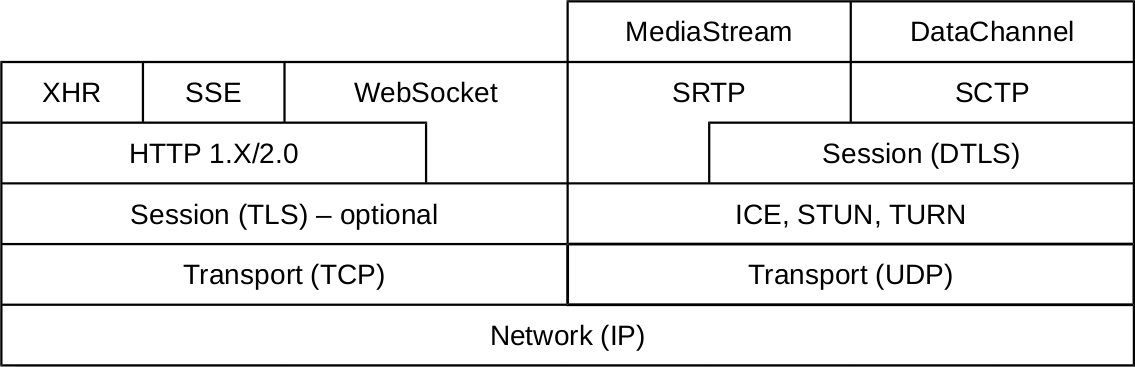
\includegraphics[width=0.9\textwidth]{figures/webrtc_stack.png}
	\caption{WebRTC protocol Stack}
\end{figure}

\ac{WebRTC} defines three main \ac{API}s: MediaStream, PeerConnection and DataChannel. 

\begin{itemize}
  \item \textbf{MediaStream} allows from the browser to access to camera, microphone and device screen. 

  \item \textbf{PeerConnection} acquires connection data and negotiates with peers.

  \item \textbf{DataChannel} allows to send whatever type of data to other peers.
\end{itemize}

\ac{WebRTC} uses \ac{UDP} for transporting data, which provides lower latencies than \ac{TCP}, but is not reliable and packet order and integrity are not assured. \ac{SCTP} and \ac{SRTP} are used for streaming data, providing a mechanism for congestion control and partial reliable delivery over \ac{UDP}. All transferred audio, data and video must be encrypted with \ac{DTLS} symmetric keys. \ac{DTLS} provides the same security guarantees as \ac{TLS}. 

\ac{TLS} doesn't support independent record decryption, for that it requires a reliable transport channel, typically \ac{TCP}. The decryption of a record depends on the previous record, which for unreliable transport protocols like \ac{UDP} may represent a problem, either due to packet loss or different reception order.

\ac{DTLS} is similar to \ac{TLS}, but on top of \ac{UDP}, the main difference is the inclusion of a sequence number per packet that is used for packet re-ordering on reception and protects from duplicated packets. If a packet sequence number is less than the expected sequence number the packet is discarded. If a packet sequence number is greater than the expected sequence number the packet may be enqueued or discarded. By knowing the sequence of messages that are sent and received in \ac{TLS}, timers are used for packet retransmission avoiding acknowledgment messages.

\begin{figure}[H]
	\centering
	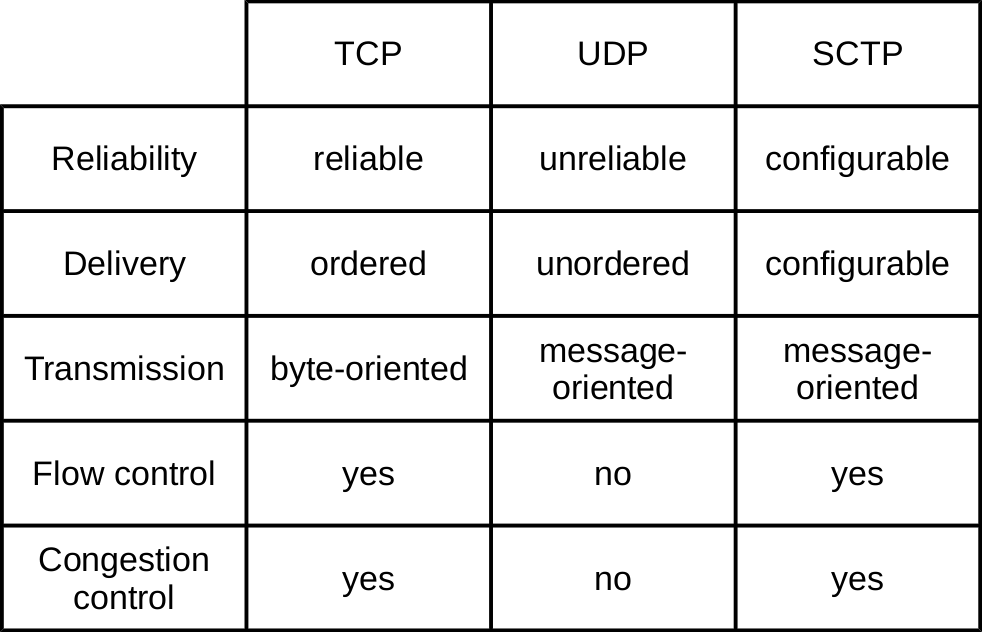
\includegraphics[width=0.6\textwidth]{figures/basic_protocols.png}
	\caption{Overview of transport protocols}
\end{figure}

\ac{WebRTC}'s \textit{DataChannel} is built on top of \ac{SCTP}, which is encapsulated by \ac{DTLS}. \ac{DTLS} encapsulation provides confidentiality, authentication and integrity over the transfered data. A \textit{Data Channel} has one incoming stream and one outgoing stream, providing bidirectional communication. Each data channel direction can be tweaked for reliable or unreliable transmission, the same can be done for order delivery and priority which can also be defined for improving the quality of service for a particular stream compared to another.

\ac{WebRTC}'s \textit{MediaStream} is built on top of \ac{SRTP}, which requires an external mechanism for key exchange. \ac{DTLS} keys are negotiated on handshake in order to achieve a secure connection. The new keys derived from \ac{DTLS} handshake are seized for \ac{SRTP} encryption, the remaining communications are done through \ac{UDP} without using \ac{DTLS}.

\textit{Skype}\footnote{\url{http://www.skype.com/}} is an application that allows video, voice and instant messaging communication over proprietary protocols, its main strength is the amount of users that are using it nowadays. But compared to \textit{Skype}, \ac{WebRTC} applications don't need to be pre-installed.

\textit{Google Hangouts}\footnote{\url{http://plus.google.com/hangouts}} is a video conference web application, in the past in order to use \textit{hangouts} on a web browser a plug-in was needed to be installed, nowadays hangouts is using \ac{WebRTC}.

Jitsi Meet\footnote{\url{http://jitsi.org/Projects/JitsiMeet}} is a \ac{WebRTC} collaborative application that uses Jitsi Videobridge for high quality and scalable video conferences and supports shared document editing. Jitsi Videobridge is a server that enables multiparty video calls.




